\documentclass[10pt,a4paper,twocolumn]{article}

\usepackage[a4paper,top=2.2cm,bottom=2cm,left=1.7cm,right=1.7cm,columnsep=0.7cm]{geometry}
\usepackage[T1]{fontenc}
\usepackage[utf8]{inputenc}
\usepackage{helvet}
\renewcommand{\familydefault}{\sfdefault}
\usepackage{amsmath,amssymb}
\usepackage{tabularx}
\usepackage{microtype}
\usepackage{booktabs}
\usepackage{graphicx}
\usepackage{enumitem}
\usepackage{fancyhdr}
\usepackage{titlesec}
\usepackage[font=small,labelfont=bf]{caption}
\usepackage[hidelinks]{hyperref}

\graphicspath{{figures/}}
\setlist{nosep,leftmargin=*}
\titleformat{\section}{\normalfont\large\bfseries\scshape}{\thesection}{0.8em}{}
\titleformat{\subsection}{\normalfont\normalsize\bfseries}{\thesubsection}{0.8em}{}
\titlespacing*{\section}{0pt}{1.2em}{0.6em}
\titlespacing*{\subsection}{0pt}{0.9em}{0.4em}

\pagestyle{fancy}
\fancyhf{}
\fancyhead[L]{\small Kaggle Project, Escola d'Enginyeria (EE), Universitat Aut\`onoma de Barcelona (UAB)}
\fancyfoot[C]{\small\thepage}
\renewcommand{\headrulewidth}{0pt}

\newcommand{\code}[1]{\texttt{\small #1}}
\renewcommand{\topfraction}{0.9}
\renewcommand{\bottomfraction}{0.8}
\renewcommand{\textfraction}{0.1}
\renewcommand{\floatpagefraction}{0.8}
\setcounter{topnumber}{3}
\setcounter{totalnumber}{5}
\renewcommand{\dbltopfraction}{0.9}
\renewcommand{\dblfloatpagefraction}{0.8}
\setcounter{dbltopnumber}{3}

\begin{document}

\noindent{\LARGE\bfseries MANGO fashion compatibility\par}
\vspace{0.6em}
\noindent{\large Francesco Tedesco\par}
\vspace{1.2em}

\noindent\textbf{Abstract} --- Recommendation systems can play a crucial role in the fashion sector by suggesting products to customers based on their potential interests. This project aims to recommend complete outfits in real time from a single input product. Each outfit is represented as one image, a variational autoencoder (VAE) learns an embedding per outfit, and random candidate outfits made of products never seen in training are ranked by their distance to the training outfits. Trained on 3,164 MANGO outfits, the model reconstructs the structure, silhouettes and dark colours of outfits; 100,000 candidates are generated and ranked in under one minute, and candidates around a single product in about two seconds. In a fill-in-the-blank evaluation on held-out outfits, the distance identifies the true product in 44\,\% of the questions and in 33\,\% of those with novel product pairs, against 25\,\% by chance: a real but modest compatibility signal, matched by colour coherence on novel pairs and far below product co-occurrence when pairs repeat. The distance also depends strongly on the darkness of the products, and the embeddings separate the two catalogues of the data.

\vspace{0.8em}
\noindent\textbf{Keywords} --- Recommendation systems, Fashion, Outfit creation, Real-time predictions, Variational Autoencoder (VAE).

\vspace{0.4em}
\begin{center}\rule{0.35\columnwidth}{0.4pt}\end{center}

\section{Introduction}

In fashion, recommendation systems can also increase sales: once it is known which product a customer is interested in, recommending a whole outfit around that product raises the probability that the customer buys one or more additional products. Two datasets are available: the first lists the products of each outfit, and the second describes each product (category, family, type, colour, material, image). Given these data, the aim of this project is to provide a solution that is useful for both the company and the customer: recommending a complete outfit based on a single input product.

\section{Methodology}

This section describes the process followed to reach the solution. The provided data are not cleaned, so data exploration and preprocessing need attention to detail. The outfits are then modelled with a convolutional autoencoder whose latent layer follows the variational autoencoder (VAE) design, in order to learn a representation of complete outfits.

\subsection{Data exploration and analysis}

A product can appear in several outfits, and every product belongs to at least one outfit. The dataset contains 7,842 outfits and 9,222 products. Counting outfits by their number of products gives Table~\ref{tab:sizes}.

\begin{table}[tb]
\centering\footnotesize
\setlength{\tabcolsep}{2.2pt}
\begin{tabular}{l*{13}{r}}
\toprule
Size & 2 & 3 & 4 & 5 & 6 & 7 & 8 & 9 & 10 & 11 & 12 & 13 & 15 \\
Outfits & 30 & 142 & 758 & 3875 & 1737 & 674 & 309 & 174 & 95 & 26 & 13 & 8 & 1 \\
\bottomrule
\end{tabular}
\caption{Number of outfits by outfit size.}
\label{tab:sizes}
\end{table}

The table shows potential outliers, such as outfits with two products or with more than ten, but a deeper analysis is needed to confirm it. Since the aim of the project is to build outfits, the analysis continues with the features that describe the class of each product. Starting with the most general description, \code{des\_product\_category}, and fixing the size to five, the most frequent sets of categories are those of Table~\ref{tab:category}.

\begin{table}[tb]
\centering\small
\begin{tabularx}{\columnwidth}{>{\raggedright\arraybackslash}Xr}
\toprule
Category set & Outfits \\
\midrule
Accessories: 3, Tops: 1, Bottoms: 1 & 1872 \\
Accessories: 4, Dress: 1 & 819 \\
Accessories: 2, Tops: 1, Outerwear: 1, Bottoms: 1 & 494 \\
Accessories: 2, Bottoms: 1, Tops: 2 & 195 \\
Accessories: 3, Bottoms: 1, Outerwear: 1 & 123 \\
\bottomrule
\end{tabularx}
\caption{Top five category sets among outfits of size five. \emph{Accessories} stands for \emph{Accesories, Swim and Intimate} and \emph{Dress} for \emph{Dresses, jumpsuits and Complete set}.}
\label{tab:category}
\end{table}

\noindent The following can be noticed:
\begin{itemize}
\item There are two base types of outfit: (1) tops + bottoms + accessories and (2) dress + accessories. In both cases an outerwear item can be added.
\item Some configurations are invalid, such as two tops in the same outfit or an outfit without a top.
\item Almost every valid outfit has more than one accessory. Since accessories include footwear, bags and jewellery, a finer description is needed.
\end{itemize}

Repeating the analysis with the subcategory \code{des\_product\_family} gives Table~\ref{tab:family}.

\begin{table}[tb]
\centering\small
\begin{tabularx}{\columnwidth}{>{\raggedright\arraybackslash}Xr}
\toprule
Family set & Outfits \\
\midrule
Footwear: 1, Jewellery: 2, Dresses: 1, Bags: 1 & 417 \\
Bags: 1, Footwear: 1, Jewellery: 1, Shirt: 1, Trousers: 1 & 164 \\
Footwear: 1, Dresses: 1, Bags: 1, Jewellery: 1, Glasses: 1 & 161 \\
Bags: 1, Jewellery: 1, Jeans: 1, T-shirt: 1, Footwear: 1 & 135 \\
Jewellery: 1, Bags: 1, Trousers: 1, Sweater: 1, Footwear: 1 & 135 \\
\bottomrule
\end{tabularx}
\caption{Top five family sets among outfits of size five.}
\label{tab:family}
\end{table}

\begin{itemize}
\item All valid outfits contain one footwear product, and they can contain accessories such as bags and glasses.
\item For tops, bottoms, dresses and outerwear this description is too specific to help build outfits.
\item Valid outfits can contain more than one product of the jewellery family, so the analysis is repeated with \code{des\_product\_type} (Table~\ref{tab:type}).
\end{itemize}

\begin{table}[tb]
\centering\small
\begin{tabularx}{\columnwidth}{>{\raggedright\arraybackslash}Xr}
\toprule
Type set & Outfits \\
\midrule
Sandals, Ring, Earrings, Dress, Handbag & 54 \\
Sandals, Earrings, Ring, Dress, Crossbody bag & 35 \\
Necklace, Handbag, Sandals, Earrings, Dress & 35 \\
Sandals, Dress, Shoulder bag, Earrings, Sunglasses & 32 \\
Sandals, Earrings, Dress, Crossbody bag, Sunglasses & 31 \\
\bottomrule
\end{tabularx}
\caption{Top five type sets among outfits of size five (one product of each type).}
\label{tab:type}
\end{table}

\begin{itemize}
\item All valid outfits contain earrings; other jewels, such as rings and necklaces, also appear in valid outfits.
\item For the remaining classes this description is too specific.
\end{itemize}

These observations define a rule for building outfits:
\begin{enumerate}
\item The base of an outfit is one of the following sets:
  \begin{itemize}
  \item Tops + Bottoms + Footwear + Earrings
  \item Dress + Footwear + Earrings
  \end{itemize}
\item The outfit can add any of the following complements, each at most once: Outerwear, Bags, Glasses, Ring and Necklace.
\end{enumerate}

A valid outfit is therefore a base plus any subset of the five complements, which gives $2 \times 2^5 = 64$ configurations. An outfit has at most nine products of different classes (eight for dress-based outfits), placed in ten class slots. The observations above hold across all outfit sizes (see the exploratory notebook); outfits of size two, or of size ten or more, never satisfy the rule.

Each image file name starts with the year of its catalogue: 4,354 products come from 2019 and 2020 and 4,868 from 2021 to 2024. No outfit combines products from both periods. Years that share an outfit therefore form one catalogue, and random outfits are created within one catalogue.

\subsection{Data processing}

Based on the rule above and on the three product descriptions, a custom product class, \code{des\_product\_class}, is derived: the family for accessories other than jewellery, the type for jewellery, and the category otherwise. This column defines the ten slots of the outfit images.

Applying the rule selects 3,164 of the 7,842 outfits; 45 of the 64 configurations occur, and the selected outfits have between three and eight products. The most frequent configuration, tops + bottoms + footwear + earrings + bag, covers 1,186 outfits. The frequency of each configuration is stored, because it is used later to create random outfits with unseen products for testing.

The next step would be to split the outfits into training and test sets. Outfits are assigned to either set stratified by configuration, and, to prevent data leakage, test outfits sharing a product with any training outfit are dropped. Products are heavily shared: 1,849 of the 4,909 products in the selected outfits appear in more than one outfit, one of them in 373. Table~\ref{tab:split} shows the consequence: with 80\,\% of the outfits for training, essentially no test outfit remains, and even with 10\,\% only about 80 do. Therefore the final model is trained on all selected outfits, and new outfits built from products that never appear in training are inspected qualitatively. The quantitative evaluation (Section~\ref{sec:evaluation}) holds out outfits instead of products.

\begin{table}[tb]
\centering\small
\begin{tabular}{rrr}
\toprule
Training share & Test outfits & Without shared products \\
\midrule
80\,\% & 633 & 0.3 \\
50\,\% & 1587 & 2.3 \\
30\,\% & 2215 & 8.2 \\
10\,\% & 2849 & 80.4 \\
\bottomrule
\end{tabular}
\caption{Test outfits, and those sharing no product with the training outfits, averaged over ten random splits stratified by configuration.}
\label{tab:split}
\end{table}

Once the training data are fixed, an auxiliary table is built with one row per outfit and one column per product class, holding the product code, or nothing when the outfit has no product of that class. Each product image is resized to $96 \times 128$ pixels (width $\times$ height) with bilinear interpolation, and the ten slots are concatenated horizontally in a fixed order (tops, bottoms, outerwear, dress, footwear, bags, glasses, earrings, ring, necklace), so every outfit becomes a $960 \times 128$ RGB image. Missing products are replaced by white images, so each class always occupies the same position. The strips are stored as JPEG images (quality 95) and decoded once at training time.

Finally, four outfits are selected to follow the training visually: two top + bottom outfits with outerwear (one also with a ring and a necklace), one with a bag and a necklace but no outerwear, and one minimal dress outfit. They show whether the model learns to place the complements around the two bases.

\subsection{Model and training process}

The encoder applies two blocks of two $3 \times 3$ convolutions (4 and 8 filters) followed by $2 \times 2$ max pooling, which reduces the image to 8 channels of $32 \times 240$. The flattened 61,440 values pass through dense layers of 512 and 256 units with ReLU activations and a linear layer of 512 units, whose outputs are split into the mean $\mu$ and the log-variance $\log\sigma^2$ of a 256-dimensional latent vector. A latent vector is sampled with the reparameterization $z = \mu + \sigma \odot \varepsilon$, $\varepsilon \sim \mathcal{N}(0, I)$. The decoder maps $z$ back to 61,440 values, reshapes them to 8 channels of $32 \times 240$, and alternates twofold nearest-neighbour upsampling with $3 \times 3$ convolutions to produce the logits of the $3 \times 128 \times 960$ image. The model has 47.5 million parameters, most of them in the two dense layers that connect to the 61,440 flattened values.

A VAE maximizes the evidence lower bound
\[
\mathrm{ELBO} = \mathbb{E}_{q(z \mid x)}\left[\log p(x \mid z)\right] - \mathrm{KL}\left(q(z \mid x) \,\|\, p(z)\right),
\]
where $q(z \mid x)$ is the variational distribution of the latent variables given an outfit and $p(z)$ is a standard normal prior. The model minimizes the negative ELBO divided by the number of pixels: the mean binary cross-entropy between the image pixels and the decoder's logits, plus the KL divergence divided by the $3 \times 128 \times 960$ pixels. The mean and log-variance come from a linear layer.

The model is implemented in PyTorch and trained on all 3,164 outfits for 400 epochs with Adam (learning rate $10^{-4}$) and seed 42, in batches of 32 outfits drawn in a new random order every epoch; the weights of the epoch with the lowest loss are kept. On an Apple M5 Pro GPU training takes 90 minutes (about 13.5 seconds per epoch). The outfit embeddings are the posterior means $\mu$ of the trained model.

Two variants are compared with this model in the evaluation: a stochastic autoencoder trained with the reconstruction term only and a ReLU after the last encoder layer (which keeps means and log-variances non-negative), and the same autoencoder with product pixels weighing five times more than the background in the loss.

\subsection{How to make the predictions}

One way to build an outfit from the embeddings of the training outfits is:
\begin{enumerate}
\item Fix an input product.
\item Try all combinations of products that form a valid outfit with it, and measure their distance to the latent space of the trained model.
\item Select the combination with the smallest distance.
\end{enumerate}

This approach is not feasible for the products that never appear in a training outfit (Table~\ref{tab:unseen}). Even for the simplest configuration, dress + footwear + earrings, there are $605 \times 139 \times 95 = 7{,}989{,}025$ combinations, and each one has to be assembled into an image, encoded and stored. Since outfits of different sizes are wanted and the customer expects an almost instant answer, the following alternative is used:

\begin{table}[tb]
\centering\small
\begin{tabular}{lr}
\toprule
Class & Unseen products \\
\midrule
Tops & 1242 \\
Bottoms & 662 \\
Dresses, jumpsuits and Complete set & 605 \\
Outerwear & 360 \\
Bags & 151 \\
Footwear & 139 \\
Earrings & 95 \\
Glasses & 58 \\
Necklace & 54 \\
Ring & 12 \\
\bottomrule
\end{tabular}
\caption{Products with an image that appear in no selected outfit, by class.}
\label{tab:unseen}
\end{table}

\begin{enumerate}
\item Set the number of outfits to create from the available products; here, 100,000 random outfits.
\item Draw a catalogue with the share of training outfits from each, then a configuration with the frequencies of that catalogue's training outfits, and one unseen product of the catalogue for each class of the configuration. Some valid configurations are never generated, but the candidates follow the distribution of the training outfits and are therefore, hopefully, close to the learned latent space.
\item Encode every candidate, building its image exactly as the training images (including the JPEG round trip). This is the most time-consuming step.
\item Compute the Euclidean distance from every candidate embedding to every training embedding.
\item Keep the minimum distance and the nearest training outfit.
\item Store a table with the product codes of each candidate, its distance and its nearest training outfit.
\item Given an input product, return the top 3 (or top $k$) candidates that contain it. This is almost instantaneous: it only filters the table, sorts it and selects the first rows.
\end{enumerate}

With this approach the company can serve outfit recommendations in real time, and add filters such as configuration, colour, material or product class. On the M5 Pro GPU, the whole procedure for 100,000 candidates takes 55 seconds.

Random candidates contain some products much more often than others: a dress appears in a median of 45 candidates and an earring in 787. For a single input product, candidates can instead be generated on demand: 1,000 candidates containing the product, from its catalogue, are generated, encoded and ranked in about two seconds.

\subsection{Evaluation}
\label{sec:evaluation}

The recommendations are also evaluated quantitatively, with a fill-in-the-blank task in which outfits, not products, are held out. 10\,\% of the outfits (314), stratified by configuration, are held out, and a model is trained on the other 2,850 for 100 epochs. For every occupied slot of a held-out outfit, the true product is compared with three decoys: products of the same class and catalogue that appear in training outfits, so that neither the catalogue nor familiarity with the product reveals the answer. A score answers a question correctly when the true product obtains the best value; random choice is right 25\,\% of the time.

The model scores are the distance to the nearest training outfit, the distance to the nearest training outfit of the same configuration, and the reconstruction error. They are compared with four baselines: the lightest option (smallest non-white share of the image), colour coherence (the share of the outfit's products in its most common colour group), co-occurrence (the number of training outfits that contain the option together with each of the outfit's other products) and random choice. Held-out outfits often share several products with a training outfit, so the questions are also evaluated on a subset of \emph{novel pairs}: questions whose true product never appears in a training outfit with any of the outfit's other products. Memorized product pairs cannot answer these questions. Intervals are 95\,\% bootstrap intervals over held-out outfits.

\section{Results and analysis}

\subsection{Training}

\begin{figure*}[t]
\centering
\begin{minipage}[b]{0.48\textwidth}\centering
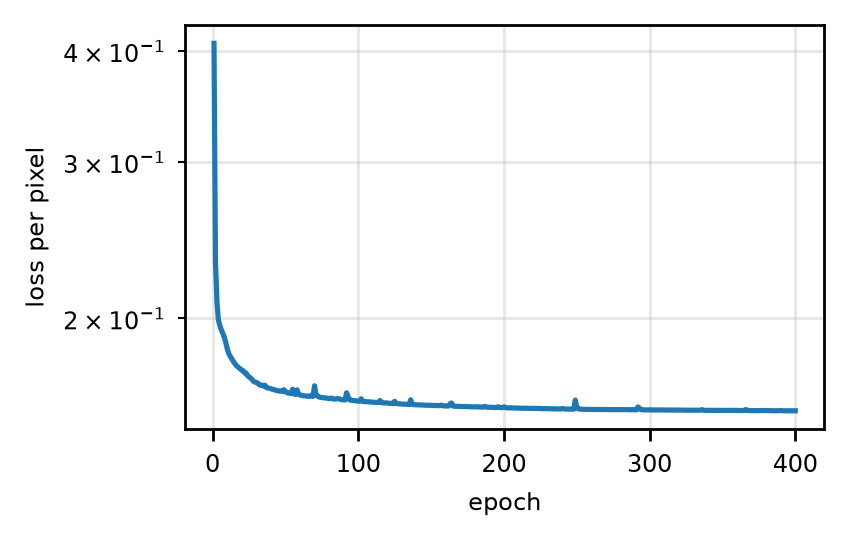
\includegraphics[width=\linewidth]{loss.png}\\{\small (a)}
\end{minipage}\hfill
\begin{minipage}[b]{0.48\textwidth}\centering
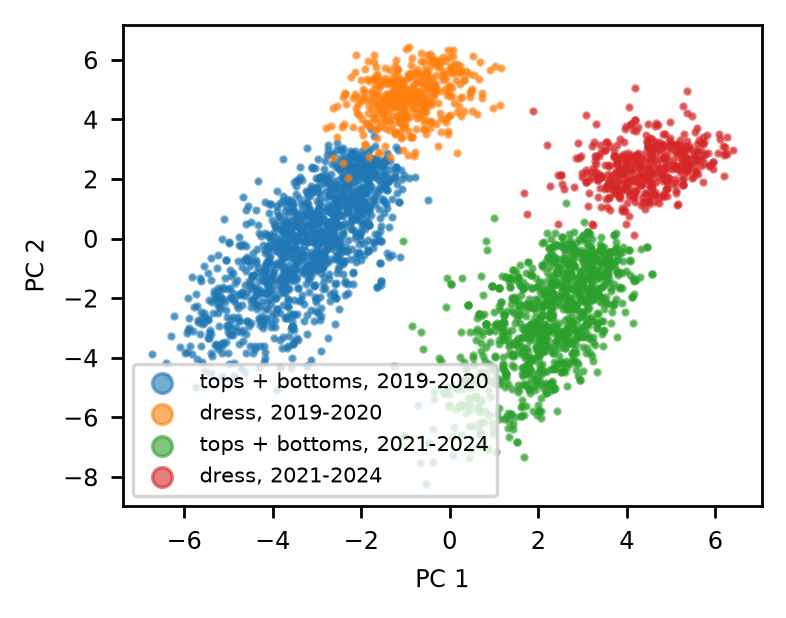
\includegraphics[width=0.9\linewidth]{latent_pca.png}\\{\small (b)}
\end{minipage}
\caption{(a) Training loss per epoch (negative ELBO per pixel, logarithmic scale). (b) Training embeddings projected on their first two principal components, by outfit base and catalogue.}
\label{fig:training}
\end{figure*}

The loss, the negative ELBO per pixel, falls from 0.408 in the first epoch to 0.185 after ten epochs and then decreases slowly (Fig.~\ref{fig:training}a), with short spikes that recover within a few epochs. It is still decreasing at the last epoch, whose weights are kept (0.1574); the improvement between epochs 100 and 400 is only 2.5\,\%.

Fig.~\ref{fig:reconstructions} compares the four sample outfits with their reconstructions from the posterior mean:
\begin{itemize}
\item The occupied slots are always reconstructed correctly: over the 31,640 slots of the training outfits, a slot is white exactly when it is empty.
\item Silhouettes and colours of dark or saturated products are reconstructed well, including some texture: the black shirt, the ankle boots, the patterned bag, the blazer, the blue jeans and the tweed jacket.
\item Light garments, such as the white shirt, the cream trousers and the white top, fade into the background, and fine prints are blurred: the printed dress keeps its colours but not its pattern.
\item Small accessories keep their position and outline (earrings, ring, necklace).
\end{itemize}

\begin{figure*}[t]
\centering
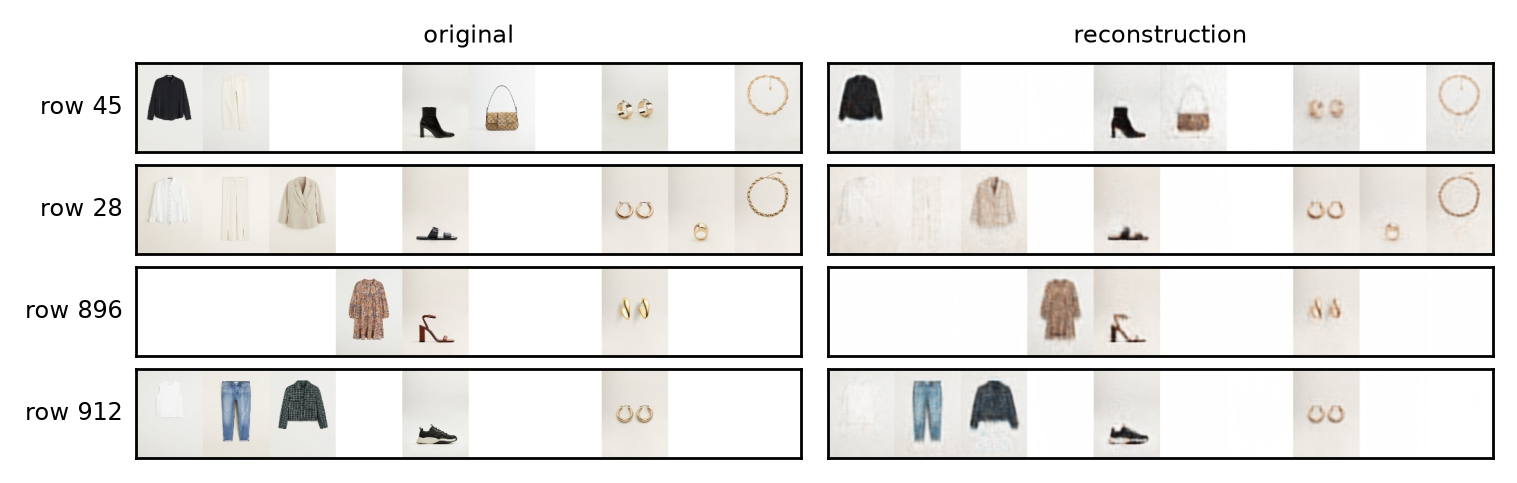
\includegraphics[width=\textwidth]{reconstructions.png}
\caption{The four sample outfits (training outfit table rows 45, 28, 896 and 912) and their reconstructions by the final model.}
\label{fig:reconstructions}
\end{figure*}

\begin{figure*}[t]
\centering
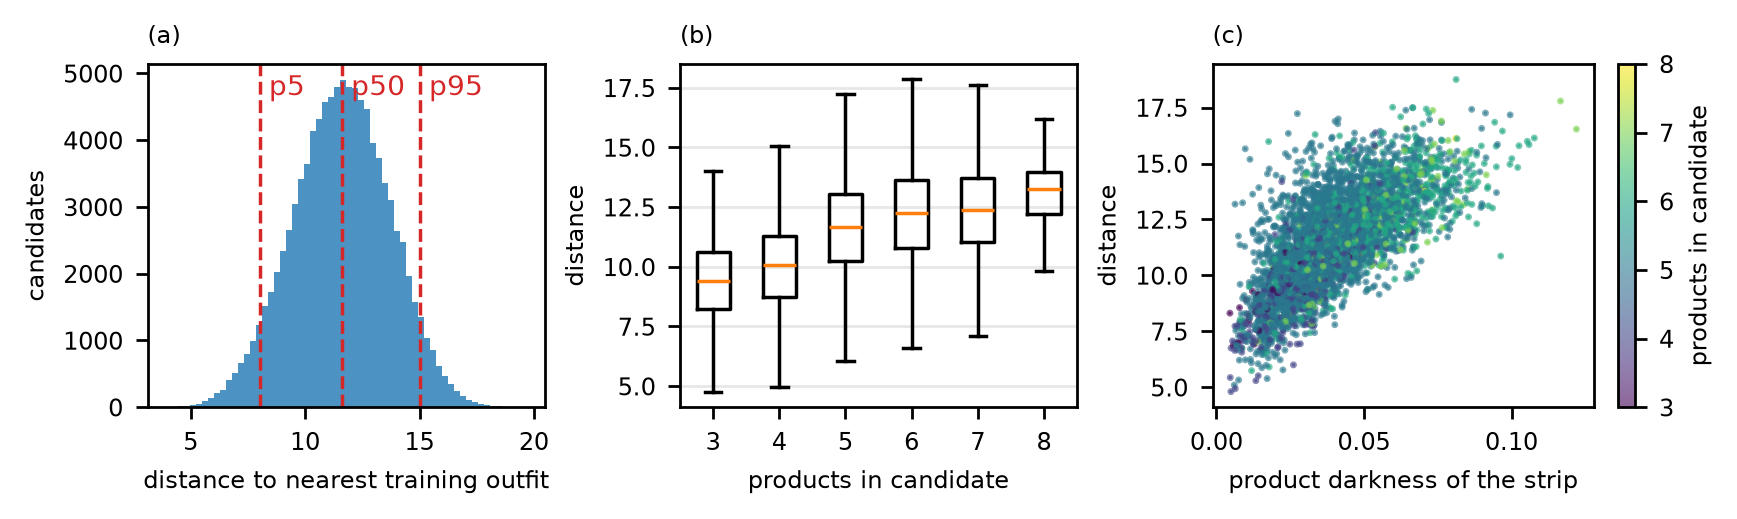
\includegraphics[width=\textwidth]{distances.png}
\caption{Distances of the 100,000 candidates to their nearest training outfit: (a) distribution; (b) by number of products (boxes: quartiles; whiskers: 1.5 interquartile ranges); (c) against the darkness contributed by product pixels (photo background excluded), for 4,000 random candidates.}
\label{fig:distances}
\end{figure*}

\begin{figure*}[t]
\centering
\begin{minipage}[t]{0.46\textwidth}\vspace{0pt}\centering
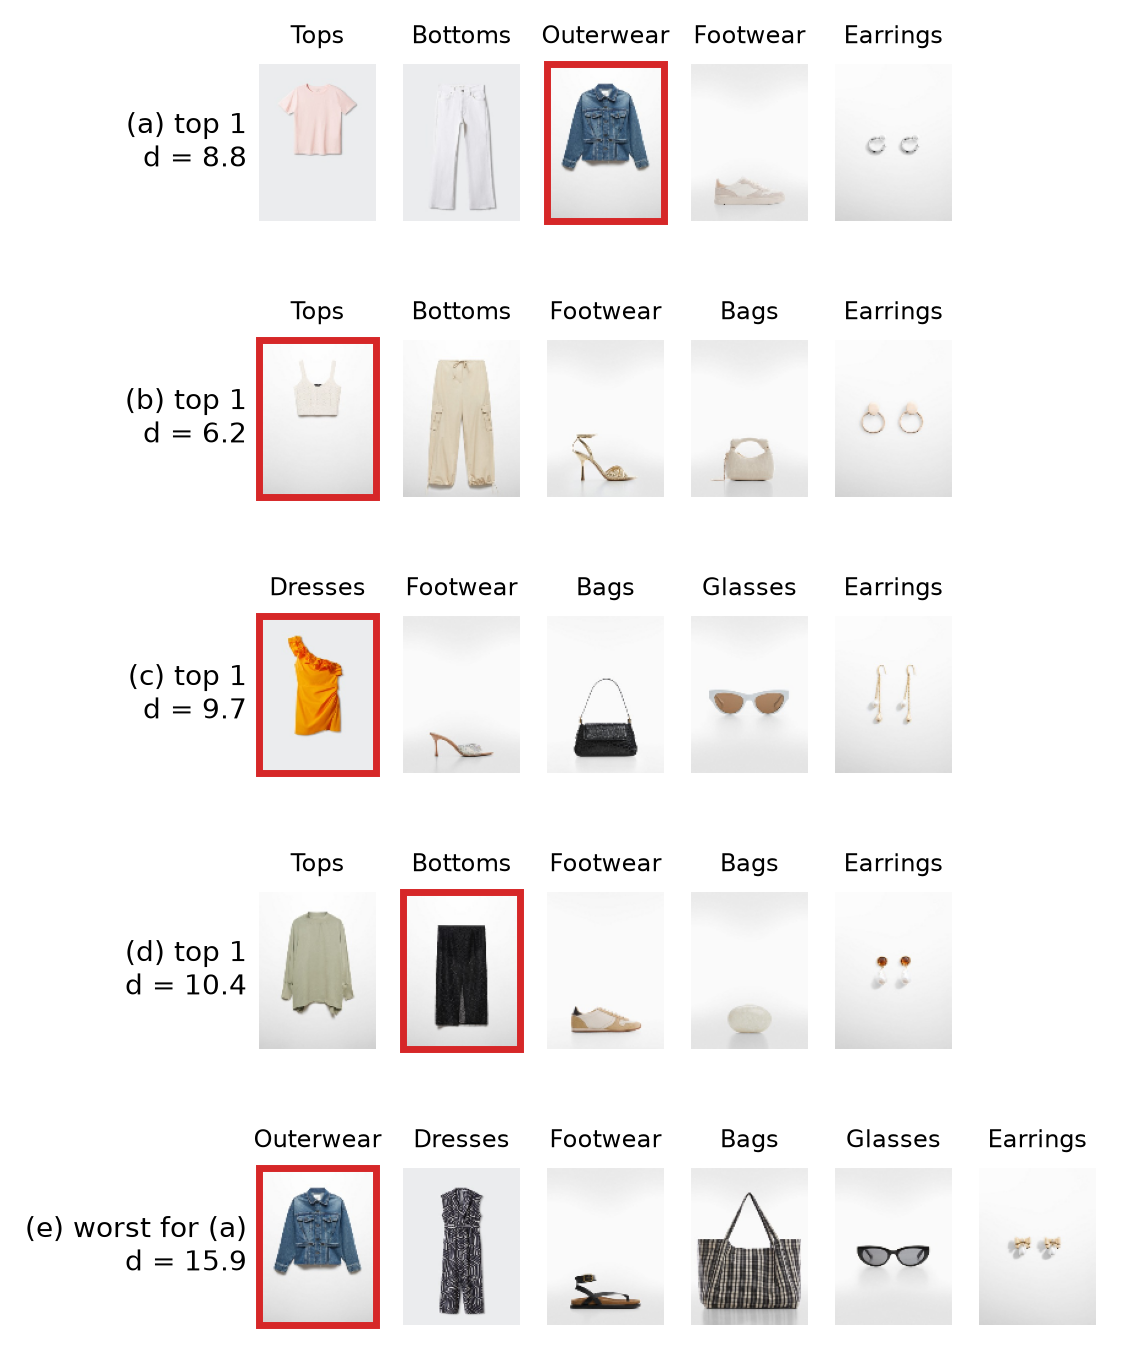
\includegraphics[width=\linewidth]{recommendations.png}
\end{minipage}\hfill
\begin{minipage}[t]{0.5\textwidth}\vspace{0pt}\centering
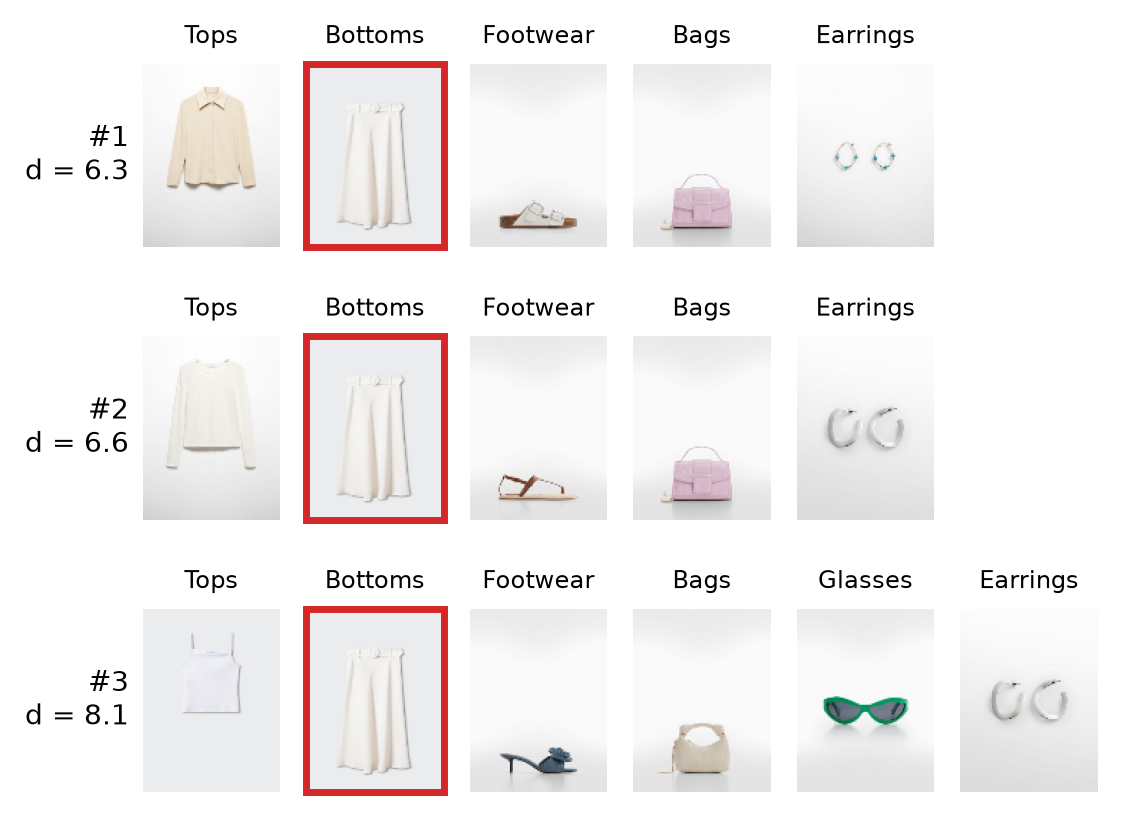
\includegraphics[width=\linewidth]{top3.png}
\end{minipage}
\caption{Left: (a)--(d) top 1 candidate for four random input products, framed in red; (e) worst candidate for the input product of (a). Right: top 3 candidates for a random white skirt. $d$ is the distance to the nearest training outfit.}
\label{fig:recommendations}
\end{figure*}

\subsection{Latent space}

The first two principal components of the 3,164 embeddings (Fig.~\ref{fig:training}b) show four well separated groups, one for each combination of outfit base and catalogue. In this projection a straight line separates dress outfits from top + bottom outfits with 99.5\,\% accuracy, and the two catalogues with 99.9\,\% (both 100\,\% in the full latent space). The catalogue difference reflects photo style and assortment rather than compatibility: the photos of the two periods differ in background tone and framing. All 256 latent dimensions are active (the variance of their posterior mean across outfits exceeds 0.01).

\subsection{Distances of the generated outfits}

Following the process described above gives the distribution of minimum distances in Fig.~\ref{fig:distances}a. It is unimodal and symmetric (skewness $-0.07$), with mean 11.6 and standard deviation 2.1; the 5th, 50th and 95th percentiles are 8.0, 11.6 and 15.0. A training outfit lies at a median distance of 10.2 from its nearest other training outfit (90th percentile: 14.1); 74.9\,\% of the candidates are farther than that median, but 87.6\,\% lie within the 90th percentile. The candidates are closest to 2,468 different training outfits.

The distance grows with the size of the candidate (Fig.~\ref{fig:distances}b): its mean goes from 9.4 for three products to 13.0 for eight, and dress outfits (11.4) are slightly closer than top + bottom outfits (11.7). It depends even more on how dark the products are. Separating product pixels from the photo background, the darkness that products contribute to the image correlates with the distance at $r = 0.69$, and between 0.64 and 0.79 within each size (Fig.~\ref{fig:distances}c). A linear model explains 8\,\% of the variance of the distance with the size alone, 30\,\% with the product area, 48\,\% with the product darkness and 3\,\% with the background darkness; 49\,\% with all four. Darker candidates have embeddings of larger norm, and the distance follows that norm closely ($r = 0.92$). Because the model reconstructs pixels, candidates with fewer, smaller or lighter products are closer to the training outfits, whatever their compatibility.

The distance also reflects colour coherence, in part. Real outfits are more coherent than candidates (on average 62.0\,\% against 46.8\,\% of their products in the most common colour group). Among candidates of the same size, the closest tenth is the most coherent (54.9\,\%); coherence then falls to about 45\,\% and rises slightly in the farthest tenth (46.5\,\%), where dark monochrome outfits sit.

\begin{table*}[t]
\centering\footnotesize
\begin{tabular}{lll}
\toprule
Score & All questions & Novel pairs \\
\midrule
\multicolumn{3}{l}{\emph{Reconstruction loss, ReLU head}} \\
\quad distance & 39.2 (35.7--42.9) & 30.5 (26.7--34.2) \\
\quad distance (same configuration) & 38.9 (35.6--42.4) & 29.4 (25.6--33.4) \\
\quad cosine distance & 39.1 (35.7--42.8) & 29.7 (25.9--33.5) \\
\quad reconstruction error & 27.8 (25.6--29.9) & 27.8 (24.6--31.1) \\
\multicolumn{3}{l}{\emph{Complete VAE (final model)}} \\
\quad distance & 44.1 (40.6--47.7) & 32.6 (28.9--36.3) \\
\quad distance (same configuration) & 43.9 (40.5--47.6) & 32.2 (28.5--36.0) \\
\quad cosine distance & 45.5 (41.9--49.1) & 32.8 (29.2--36.6) \\
\quad reconstruction error & 28.0 (25.8--30.2) & 25.7 (22.6--29.0) \\
\multicolumn{3}{l}{\emph{Reconstruction loss, ReLU head, foreground weight 5}} \\
\quad distance & 44.1 (40.6--47.7) & 30.6 (27.0--34.4) \\
\quad distance (same configuration) & 43.4 (40.0--47.0) & 29.3 (25.3--33.0) \\
\quad cosine distance & 45.0 (41.4--48.8) & 31.4 (27.6--35.4) \\
\quad reconstruction error & 27.9 (25.6--30.1) & 26.1 (23.0--29.3) \\
\multicolumn{3}{l}{\emph{Baselines}} \\
\quad co-occurrence & 57.3 (54.6--60.2) & 17.7 (16.7--18.5) \\
\quad colour coherence & 33.4 (31.5--35.1) & 32.2 (29.4--35.0) \\
\quad lightest option & 24.2 (22.0--26.4) & 25.9 (22.4--29.0) \\
\quad random & 24.2 (22.1--26.3) & 22.8 (19.7--26.1) \\
\bottomrule
\end{tabular}

\caption{Fill-in-the-blank accuracy in \% with 95\,\% bootstrap intervals: 1,616 questions on 314 held-out outfits, 711 of them novel pairs. Each question has four options, so random choice is right 25\,\% of the time. The models are trained for 100 epochs on the other 2,850 outfits.}
\label{tab:evaluation}
\end{table*}

\subsection{Recommendations}

The analysis of recommendations starts with the best candidate (top 1) for random input products; the top 3 candidates of a product share few products besides the input (0.10 on average). Fig.~\ref{fig:recommendations} (left, a--d) shows four examples, with the input product framed in red:
\begin{itemize}
\item (a) A denim jacket: a pink T-shirt, white jeans, white trainers and small silver earrings, a classic casual outfit.
\item (b) A cream knitted top: beige cargo trousers, gold sandals, a cream bag and earrings, a consistent neutral palette.
\item (c) An orange one-shoulder dress: clear heeled mules, a black bag, white sunglasses and pearl earrings, an evening outfit with a contrasting bag.
\item (d) A black skirt: a sage blouse, beige trainers, a pearl clutch and white earrings; the colours work, but trainers and a pearl clutch are an unusual mix.
\end{itemize}

The worst candidate for the denim jacket of example (a) is shown in Fig.~\ref{fig:recommendations}e: a black-and-white printed jumpsuit with a plaid tote, black sandals and sunglasses. Its two clashing patterns make it a poor outfit, and its large distance (15.9) is also consistent with the darkness effect: it has six products and large dark areas.

Fig.~\ref{fig:recommendations} (right) shows the top 3 candidates for a random white skirt. All three are light summer outfits: a cream shirt or a white top, flat or low sandals, light bags and silver or beaded earrings; the first two share the same pink bag.

\subsection{Quantitative evaluation}

Table~\ref{tab:evaluation} lists the accuracy of every score. Co-occurrence is by far the strongest score on all questions (57.3\,\%): held-out outfits often repeat product pairs of training outfits. On novel pairs it falls below chance, as expected, because decoys that ever appeared with the outfit's products always win.

The complete VAE is the best model. Its distance answers 44.1\,\% of all questions and 32.6\,\% of the novel pairs, against 39.2\,\% and 30.5\,\% for the reconstruction-only model. Weighting product pixels helps on all questions (44.1\,\%) but not on novel pairs (30.6\,\%), so it mostly improves the recognition of near-duplicates. The distance to training outfits of the same configuration and the cosine distance perform like the plain distance, since the four options of a question share their configuration and differ in one product. The reconstruction error and the lightest option are close to chance: within a question, the model does not simply prefer lighter outfits.

On novel pairs, the visual signal is modest: the best model is about 8 points above chance, and a simple colour-coherence rule (32.2\,\%) is as accurate. The image embeddings therefore capture compatibility beyond memorized pairs, but little more than colour.

\section{Conclusions}

This project delivers a working solution for both the company and the customer: candidate outfits are created offline or around a single product within a few seconds, and recommending is a lookup that can be served in real time. The complete VAE reconstructs the structure, silhouettes and dark colours of outfits, and its embeddings are organized first by outfit base and by catalogue. In the fill-in-the-blank evaluation, its distance recognizes the true product in 44\,\% of the questions and in 33\,\% of those with novel product pairs, against 25\,\% for random choice. This is clear but modest evidence of compatibility: memorized co-occurrence is much stronger when product pairs repeat, colour coherence is as good on novel pairs, and the distance across candidates of different sizes still depends strongly on the darkness of their products. The recommendations are promising, but the score needs better visual features and should be combined with co-occurrence and colour before it is used.

\section{Next steps}

\begin{enumerate}
\item \textbf{Combine the signals.} Co-occurrence, colour coherence and visual distance capture different information. Train a ranker on fill-in-the-blank questions built from training outfits and evaluate it on the held-out ones.
\item \textbf{Better visual features.} Replace raw pixels with per-product features from an image encoder pretrained on fashion images, or normalize the photo backgrounds, so that the embeddings depend less on photo style (catalogue) and product darkness.
\item \textbf{A ranking independent of size and darkness.} Within a question all options share a configuration, so the evaluation does not test the ranking of candidates of different sizes. Extend it, for example by comparing held-out outfits with random candidates of other configurations, and normalize the distance accordingly.
\item \textbf{Tune the model.} Combine the complete VAE with foreground weighting, vary the KL weight and the number of epochs, and evaluate each setting with the same questions.
\item \textbf{Human evaluation.} Ask stylists to rate top-ranked and random candidates, to check that the fill-in-the-blank accuracy reflects perceived compatibility.
\item \textbf{More data and metadata.} Relax the outfit rules to train on more outfits, and give the model colour, fabric and category metadata as inputs.
\item \textbf{Serving.} Expose the on-demand recommendation through an API with filters for configuration, colour and material.
\end{enumerate}

\end{document}
